% Author: Izaak Neutelings (December 2020)
\documentclass[border=3pt,tikz]{standalone}
\usepackage{physics}
\usepackage{tikz}
\usetikzlibrary{calc} % for pic
\usetikzlibrary{angles,quotes} % for pic (angle labels)
%\usetikzlibrary{arrows.meta} % for arrow size
\tikzset{>=latex} % for LaTeX arrow head
\usepackage[outline]{contour} % glow around text
\contourlength{1.2pt}

\colorlet{xcol}{blue!70!black}
\colorlet{vcol}{green!60!black}
\colorlet{myred}{red!65!black}
\colorlet{metalcol}{blue!25!black!30!white}
\tikzstyle{vvec}=[->,vcol,very thick,line cap=round]
\tikzstyle{force}=[->,myred,thick,line cap=round]
\tikzstyle{Fproj}=[->,myred!50,thick,line cap=round]
\tikzstyle{rope}=[brown!30!black,double=brown!90!black,double distance=1.2,line width=0.4,line cap=round]
\tikzstyle{dark rope}=[brown!10!black,double=brown!60!black,double distance=1.2,line width=0.4]
\tikzstyle{metal}=[draw=metalcol!10!black,rounded corners=0.1,
  top color=metalcol,bottom color=metalcol!80!black,shading angle=10]
\tikzstyle{wood}=[draw=brown!80!black,rounded corners=0.1,
  top color=brown!80,bottom color=brown!80!black!80,shading angle=10]
\tikzstyle{width}=[<->] %{Latex[length=4,width=3]}-{Latex[length=4,width=3]}]
\newcommand{\vbF}{\vb{F}}
\def\wave#1#2{
  ({(#1-0.36)*\xmax},0) to[out=0,in=180,looseness=1] (#1*\xmax,#2*\A)
  to[out=0,in=180,looseness=1]++ (0.36*\xmax,#2*-\A)
}

\begin{document}

% VELOCITY - FORCES
\def\xmax{3.0}
\def\A{0.8}
\def\t{0.12}
\def\v{0.25*\xmax}
\def\R{0.60*\A}
\def\FT{0.7*\A} % tension
\def\Ft{0.8*\A} % tangential tension
\def\Fr{0.4*\A} % tension
\begin{tikzpicture}
  \coordinate (T) at (0,\A);
  \coordinate (L) at (-0.6*\xmax,0);
  \coordinate (R) at (0.6*\xmax,0);
  
  % STRING
  \draw[dashed,thin] (0,\A-\R) circle(\R);
  \draw[rope] (-\xmax,0) -- \wave{0}{1} -- (\xmax,0);
  \draw[force] (T) --++ (-\Ft,0) node[above=1,left=-3] {$\vbF_\mathrm{t}$};
  \draw[force] (T) --++ ( \Ft,0) node[above=1,right=-2] {$\vbF_\mathrm{t}$};
  \draw[force] (T) --++ (0,-\Fr) node[below] {\contour{white}{$\vbF_\mathrm{r}$}};
  \draw[force] (L) --++ (-\FT,0) node[below] {$\vbF$};
  \draw[force] (L) --++ ( \FT,0) node[below] {$\vbF$};
  \draw[force] (R) --++ (-\FT,0) node[below] {$\vbF$};
  \draw[force] (R) --++ ( \FT,0) node[below] {$\vbF$};
  \fill (T) circle(0.04);
  \fill (L) circle(0.04);
  \fill (R) circle(0.04);
  
  % ENDS
  \draw[metal] (-\xmax,0) circle(0.7*\t);
  \draw[metal] ( \xmax,0) circle(0.7*\t);
  \draw[wood] (-\xmax,-0.5*\A) rectangle++ (-\t,1.8*\A);
  \draw[wood] ( \xmax,-0.5*\A) rectangle++ ( \t,1.8*\A);
  \draw[vvec] (T)++(-42:0.6*\A) --++ (\v,0) node[below=0,right=-2] {$v$};
  
\end{tikzpicture}


% VELOCITY - FORCES - zoom
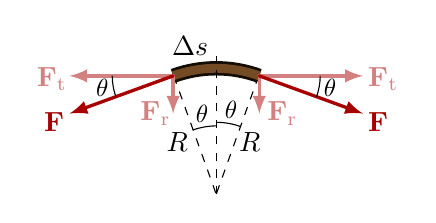
\begin{tikzpicture}
  \def\A{1.6}
  \def\xmax{10}
  \def\ang{20}
  \def\F{1.4} % tension
  \coordinate (O) at (0,0);
  \coordinate (L) at (90+\ang:\A);
  \coordinate (R) at (90-\ang:\A);
  \draw[dashed]
    (L)++( 0.008,0) -- (O) node[pos=0.56,left] {$R$}
    (R)++(-0.008,0) -- (O) node[pos=0.56,right=-2] {$R$};
  \draw[dark rope,double distance=3.2,line width=1.0]
    (L) arc(90+\ang:90-\ang:\A);
  %\node[above left] at ({(\xb+\xa)/2},{\A*cos(\om*(\xb+\xa)/2)}) {$\dd{m}$};
  \node[above left=1] at (90-0.1*\ang:\A) {$\Delta s$};
  \draw[Fproj,very thick] (L) --++ ({-\F*cos(\ang)},0)
    coordinate (LX) node[below=1,left=-3] {$\vbF_\mathrm{t}$};
  \draw[Fproj,very thick] (L) --++ (0,{-\F*sin(\ang)}) node[above=0,left=-3] {$\vbF_\mathrm{r}$};
  \draw[force,very thick] (L) --++ (180+\ang:\F)
    coordinate (LT) node[below=3,left=-2] {$\vbF$};
  \draw[Fproj,very thick] (R) --++ ({ \F*cos(\ang)},0)
    coordinate (RX) node[below=1,right=-2] {$\vbF_\mathrm{t}$};
  \draw[Fproj,very thick] (R) --++ (0,{-\F*sin(\ang)}) node[above=0,right=-1] {$\vbF_\mathrm{r}$};
  \draw[force,very thick] (R) --++ (-\ang:\F)
    coordinate (RT) node[below=3,right=-2] {$\vbF$};
  \draw[dashed] (O) -- (0,1.1*\A) coordinate (T);
  \draw pic[-,"$\theta$"{scale=0.9},draw=black,angle radius=22,angle eccentricity=1.18]
    {angle=LX--L--LT};
  \draw pic[-,"$\theta$"{scale=0.9},draw=black,angle radius=22,angle eccentricity=1.18]
    {angle=RT--R--RX};
  \draw pic[-,"$\theta$"{scale=0.9},draw=black,angle radius=24.7,angle eccentricity=1.19]
    {angle=T--O--L};
  \draw pic[-,"$\theta$"{scale=0.9},draw=black,angle radius=26,angle eccentricity=1.19]
    {angle=R--O--T};
\end{tikzpicture}


% TENSION
\def\xmax{3.0}
\def\A{0.6}
\def\v{0.25*\xmax}
\def\F{0.8*\A} % tension
\def\om{360/\xmax} % omega (degrees)
\begin{tikzpicture}
  \def\xa{0.88*\xmax}
  \def\xb{0.95*\xmax}
  \coordinate (T) at (0,\A);
  \draw[width] (1.15*\xmax,-\A) node[right,scale=0.9] {$x$} -|++ (-0.7*\A,0.7*\A) node[left,scale=0.9] {$y$};
  \draw[rope,samples=100,smooth,variable=\x,domain=0:\xmax]
    plot(\x,{\A*cos(\om*\x)});
  \draw[dark rope,samples=100,smooth,variable=\x,domain=\xa:\xb]
    plot(\x,{\A*cos(\om*\x)});
  \draw[force] (\xa,{\A*cos(\om*\xa)}) --++ ({-atan(\A*2*pi/\xmax*sin(\om*\xa))-180}:\F)
    node[above left=-2] {$\vbF_1$};
  \draw[force] (\xb,{\A*cos(\om*\xb)}) --++ ({-atan(\A*2*pi/\xmax*sin(\om*\xb))}:\F)
    node[below right=-2] {$\vbF_2$};
  %\draw[force] (L) --++ (-\FT,0) node[below] {$\vbF$};
  %\draw[force] (L) --++ ( \FT,0) node[below] {$\vbF$};
  %\draw[vvec] (T)++(-48:0.7*\A) --++ (\v,0) node[right=-2] {$v$};
\end{tikzpicture}

% TENSION - zoom
\begin{tikzpicture}
  \def\A{2.2}
  \def\xmax{10}
  \def\xa{0.87*\xmax}
  \def\xb{0.95*\xmax}
  \def\F{1.2} % tension
  \coordinate (L) at (\xa,{\A*cos(\om*\xa)});
  \coordinate (R) at (\xb,{\A*cos(\om*\xb)});
  \draw[dark rope,double distance=3.2,line width=1.0,samples=50,smooth,variable=\x,domain=\xa:\xb]
    plot(\x,{\A*cos(\om*\x)});
  \node[above left] at ({(\xb+\xa)/2},{\A*cos(\om*(\xb+\xa)/2)}) {$\dd{m}$};
  \draw[force,very thick] (\xa,{\A*cos(\om*\xa)}) --++ ({-atan(\A*2*pi/\xmax*sin(\om*\xa))-180}:\F)
    coordinate (T1) node[above=0,left=-2] {$\vbF_1$};
  \draw[force,very thick] (\xb,{\A*cos(\om*\xb)}) --++ ({-atan(\A*2*pi/\xmax*sin(\om*\xb))}:\F)
    coordinate (T2) node[above=0,right=-2] {$\vbF_2$};
  \draw[dashed]
    (L) --++ (-\F,0) coordinate (X1)
    (R) --++ ( \F,0) coordinate (X2);
  \draw[width] (L)++({-atan(\A*2*pi/\xmax*sin(\om*\xa))-101}:0.1) --++ (\xb-\xa,0)
    node[midway,below] {$\dd{x}$};
  \draw[width] (R)++({-atan(\A*2*pi/\xmax*sin(\om*\xb))-79}:0.1) --++ (0,{\A*cos(\om*\xa)-\A*cos(\om*\xb)})
    node[midway,right] {$\dd{y}$};
  \draw pic[-,"$\theta_1$"{scale=1},draw=black,angle radius=13,angle eccentricity=1.4]
    {angle=X1--L--T1};
  \draw pic[-,"\contour{white}{$\theta_2$}"{scale=1,below=-5},draw=black,angle radius=14,angle eccentricity=1.5]
    {angle=X2--R--T2};
\end{tikzpicture}


\end{document}